Despite its ubiquity across human culture, music making is not easily accessible. Traditional instruments such as the piano, guitar, and violin require the performer to have a high level of manual dexterity in order to perform the instrument properly. This presents a challenge to people with disabilities, notably those with motor impairments. Recent research has addressed this problem, introducing new approaches to music making through the use of digital musical instruments, such as prosthetic devices, mouth-operated controllers, touchscreen controllers, and mouse-controlled interfaces \cite{15}.

The intersection of human-computer interaction (HCI), interactive music, and brain-computer interfaces (BCIs) has manifested in the creation of music-specific BCIs, also known as brain-computer music interfaces (BCMIs). BCMIs have been designed for numerous applications, such as musical neurofeedback \cite{2}, music composition \cite{3}, and special needs \cite{1}. Recently, BCMIs have been widely used for music performance applications \cite{5, 8, 7, 6, 3, 10, 9}. Through direct interaction with the human brain, BCMIs provide direct affective components (such as musical neurofeedback) to music performance and directly generate musical ideas from EEG signals through sonification. Though these approaches introduce great artistic, compositional, and experimental value, the use of such BCMIs for accessible applications may imply a steep learning curve, as these systems may be hard to set up or difficult to understand for a novice musician. In addition, some of these systems are designed for medical or research grade EEG devices \cite{3, 10, 8}, making affordability an issue when considering widespread use. 

A brain-computer interface that uses facial expression signals reduces the learning curve typically introduced by motor imagery (MI) systems, since MI EEG data requires significant user concentration to generate \cite{inMIdefense3}, and the generation of MI EEG activity has been found to be challenging for many users \cite{inMIdefense1}. While computer vision can be used to detect facial expressions, capturing facial expressions using EEG devices overcomes the need for a camera facing the user’s face, adequate light conditions, optimal pose/angle, etc \cite{facialexpressionpaper2,facialexpressionpaper}.

Because facial expression detection only introduces the ability to send discrete commands, a separate method for extracting continuous control was used. MusEEG is able to send continuous band power data of the theta (4 - 8 Hz),  alpha (8 - 12 Hz), beta (12 - 30 Hz) and gamma (30 - 60 Hz) bands. Previous research indicates that band-specific activity contains valuable cognitive information. Beta activity has been associated with psychological and physical stress, whereas theta and low alpha activity has been associated with response inhibition and attentional demands such as phasic (event-related) alertness \cite{alphabeta, overallbandpaper}. High alpha activity is related to task performance in terms of speed, relevance and difficulty \cite{alphatheta}, and gamma activity reflects complex cognitive functions such as multimodal processing and object representation \cite{gamma}. Using affective data to control musical parameters gives the performer the option to create a direct link between the performer’s cognitive state and the music being performed.

The purpose of MusEEG is to reduce the accessibility gap present in music performance by introducing a musical instrument that not only is accessible to people who possess severe motor disabilities, but also provides a plug-and-play interface with different levels of musical abstraction, allowing for people with little musical experience to be able to make music. 

\pagebreak

\section{Background}
\subsection{Electroencephalography}
Electroencephalography (EEG) is the process of measuring electrical activity (voltage
fluctuations) in different parts of the brain. It is a noninvasive procedure, performed by placing
multiple electrodes along the scalp at specific measurement points. Although EEG is typically
used to diagnose epilepsy, sleep disorders, and other conditions, new studies have found EEG
signals viable for data collection of human activity, such as gestures and other motor imagery.
This study makes use of an EEG-based brain-computer interface (BCI). Brain-
computer interfaces are systems that enable the central nervous system of a person to send
control signals to a given electronic device. The EEG device used in this study is
the Emotiv® EPOC+, a commercially available neuroheadset. The Emotiv® EPOC+ consists of 16
electrodes placed strategically along the scalp. 2 of these electrodes are used as reference
sensors, while the other 14 are responsible for recording brain waves. Brain waves are a way of
classifying the voltage fluctuations in the brain into a spectrum of multiple wave frequency
ranges, such as delta (0.5 - 4 Hz), theta (4 - 8 Hz), alpha (8 - 12 Hz), beta (12 - 30 Hz) and
gamma (30 - 60 Hz). A conductive saline solution or gel is applied prior to placing the
neuroheadset on the subject to decrease the impedance between the electrodes and the scalp, thus improving the EEG signal quality.

\subsection{Artificial Neural Networks}
Artificial Neural Networks (ANN, commonly referred to as neural networks) are computational structures based on the human brain. A neural network operates as a “massively parallel distributed processor” made up of single processing units (neurons) \cite{annbook}. Neural networks consist of three different types of layers: an input layer, an output layer, and multiple hidden (processing) layers. Each layer consists of a parallel column of neurons, and neurons from one layer are connected to neurons from the previous and following layers. 
Each neuron receives multiple inputs from the previous layer of neurons. Each of these inputs have assigned synaptic weights by which the inputs are multiplied. A bias value is then added to the neuron, which is then added, along with the weighted inputs, to a central summing junction. The resulting value is then passed through an activation function which normalizes the amplitude range of each neuron. A nonlinear model of a neuron can be observed in  (Figure~\ref{fig:neuron}).
 
\begin{figure}[H]
	\centering
		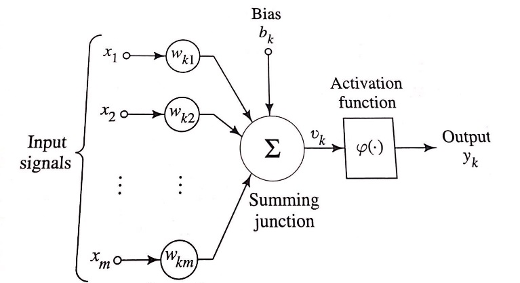
\includegraphics[width=0.6\columnwidth]{neuron.png}
	\caption{Non-linear model of a neuron \cite{annbook}}
	\label{fig:neuron}
\end{figure} 

Neural networks are great at performing classification tasks. They take a set of input data and map such input to a specific output. This is a desirable trait for facial expression classification, as an input (brain signal) should be mapped to a certain output (facial expression). 


